\documentclass[journal]{IEEEtran}
\usepackage[a5paper, margin=10mm, onecolumn]{geometry}
%\usepackage{lmodern} % Ensure lmodern is loaded for pdflatex
\usepackage{tfrupee} % Include tfrupee package

\setlength{\headheight}{1cm} % Set the height of the header box
\setlength{\headsep}{0mm}     % Set the distance between the header box and the top of the text

\usepackage{gvv-book}
\usepackage{gvv}
\usepackage{cite}
\usepackage{amsmath,amssymb,amsfonts,amsthm}
\usepackage{algorithmic}
\usepackage{graphicx}
\usepackage{textcomp}
\usepackage{xcolor}
\usepackage{txfonts}
\usepackage{listings}
\usepackage{enumitem}
\usepackage{mathtools}
\usepackage{gensymb}
\usepackage{comment}
\usepackage[breaklinks=true]{hyperref}
\usepackage{tkz-euclide} 
\usepackage{listings}
% \usepackage{gvv}                                        
\def\inputGnumericTable{}                                 
\usepackage[latin1]{inputenc}                                
\usepackage{color}                                            
\usepackage{array}                                            
\usepackage{longtable}                                       
\usepackage{calc}                                             
\usepackage{multirow}                                         
\usepackage{hhline}                                           
\usepackage{ifthen}                                           
\usepackage{lscape}
\begin{document}

\bibliographystyle{IEEEtran}
\vspace{3cm}

\title{10.3.1.1}
\author{EE24BTECH11052 - Rongali Charan}
 \maketitle
% \newpage
% \bigskip
{\let\newpage\relax\maketitle}

\renewcommand{\thefigure}{\theenumi}
\renewcommand{\thetable}{\theenumi}
\setlength{\intextsep}{10pt} % Space between text and floats


\numberwithin{equation}{enumi}
\numberwithin{figure}{enumi}
\renewcommand{\thetable}{\theenumi}


\textbf{Question:}\\
Solve the following pairs of equations by reducing them to a pair of linear equations:
\begin{align*}
    \frac{5}{x-1} + \frac{1}{y-2} &= 2\\
    \frac{6}{x-1} - \frac{3}{y-2} &= 1
\end{align*}

\textbf{Solution:}\\
Let's solve this using LU decomposition. First, let's substitute:
\begin{align}
    \frac{1}{x-1} &= u\\
    \frac{1}{y-2} &= v
\end{align}

Then our equations become:
\begin{align}
    5u + v &= 2 \label{eq1}\\
    6u - 3v &= 1 \label{eq2}
\end{align}

This can be written in matrix form as:
\begin{align}
    \myvec{5 & 1\\6 & -3}\myvec{u\\v} = \myvec{2\\1}
\end{align}

Any non-singular matrix can be represented as a product of a lower triangular matrix $L$ and an upper triangular matrix $U$
\begin{align}
    A\vec{x} = LU\vec{x} = \vec{b}
\end{align}

The upper triangular matrix $U$ is found by row reducing $A$:
\begin{align}
    \myvec{5 & 1\\6 & -3} \xrightarrow{R_2 \rightarrow R_2 - \frac{6}{5}R_1} \myvec{5 & 1\\0 & -\frac{21}{5}}
\end{align}
Let 
\begin{align}
    L = \myvec{1 & 0\\ l_{21} & 1}
\end{align}
$l_{21}$ is the multiplier used to zero $a_{21}$, so $l_{21} = \frac{6}{5}$.\\
\newline
\begin{align}
    L = \myvec{1 & 0\\\frac{6}{5} & 1}
\end{align}

Now,
\begin{align}
    A = \myvec{5 & 1\\6 & -3} = \myvec{1 & 0\\\frac{6}{5} & 1}\myvec{5 & 1\\0 & -\frac{21}{5}}
\end{align}

We can solve this using two steps:
\begin{align}
    L\vec{y} = \vec{b}\\
    U\vec{x} = \vec{y}
\end{align}

Using forward substitution:
\begin{align}
    \myvec{1 & 0\\\frac{6}{5} & 1}\myvec{y_1\\y_2} = \myvec{2\\1}
\end{align}

This gives:
\begin{align}
    y_1 &= 2\\
    \frac{6}{5}(2) + y_2 &= 1\\
    y_2 &= -\frac{7}{5}
\end{align}

Now using back substitution:
\begin{align}
    \myvec{5 & 1\\0 & -\frac{21}{5}}\myvec{u\\v} = \myvec{2\\-\frac{7}{5}}
\end{align}

This gives:
\begin{align}
    v &= \frac{1}{3}\\
    5u + \frac{1}{3} &= 2\\
    u &= \frac{1}{3}
\end{align}

Therefore:
\begin{align}
    \frac{1}{x-1} = \frac{1}{3} &\implies x = 4\\
    \frac{1}{y-2} = \frac{1}{3} &\implies y = 5
\end{align}

The solution is:
\begin{align}
    \myvec{x\\y} = \myvec{4\\5}
\end{align}

\begin{figure}[h!]
   \centering
	 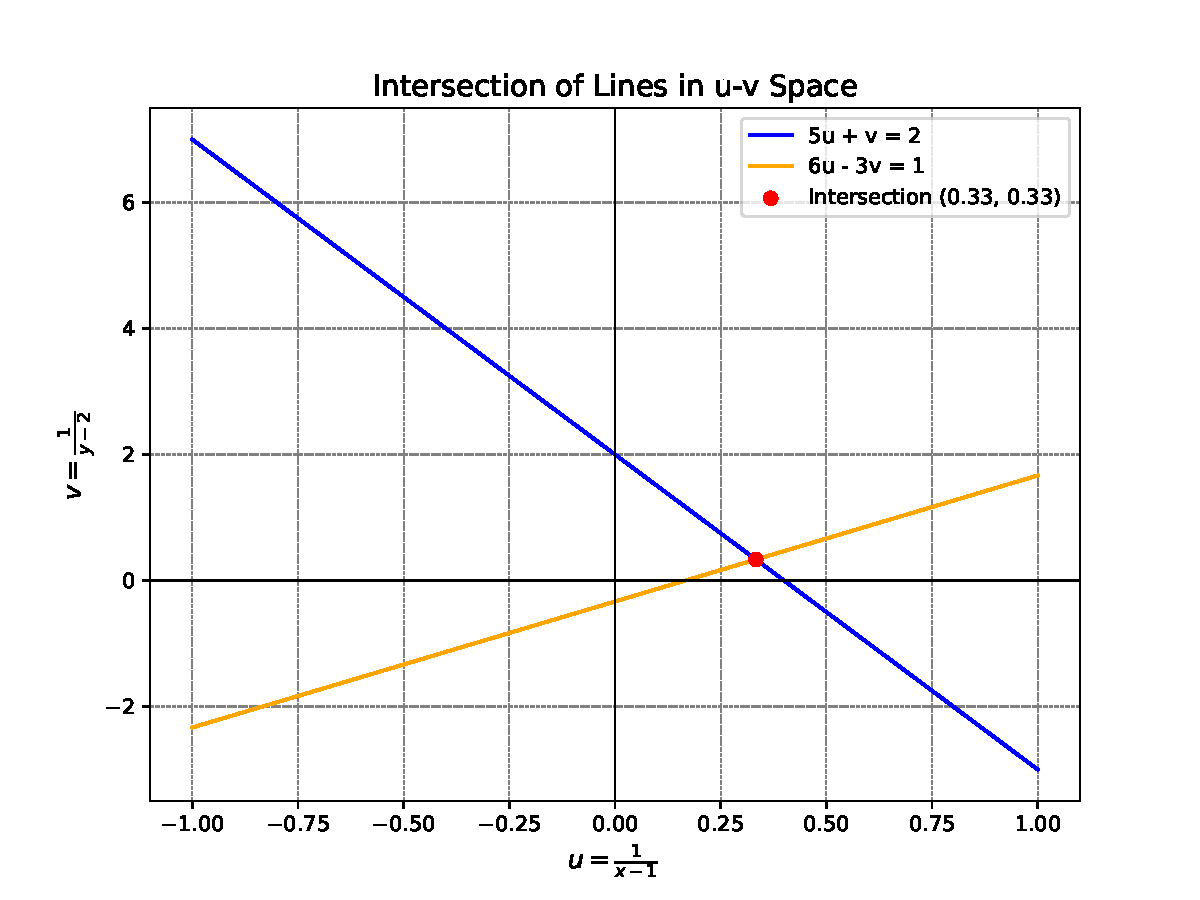
\includegraphics[width=\textwidth]{figs/fig.pdf}
   % Add your figure here if needed
   \caption{Graph of the solution}
\end{figure}

\end{document}
